\begin{remark}
    Section made from lectures done by Kjellmar Oksavik. Other sources are \citet{BrekkeAsgeir2013Potu} --- chapter 1.
\end{remark}
\section{The solar atmosphere}
The temperature at the solar center is assumed to be as high as \(\num{1.5e7}\) K. At this high temperature protons will be converted to helium nuclei by thermonuclear reactions such as the proton–proton and carbon-cycle chains. The proton-proton chain can be illustrated as
\begin{align*}
    \pres{1}{}{H}+\pres{1}{}{H}&\rightarrow \pres{2}{}{H}+e^++\nu+\SI{0.42}{\mega\electronvolt}\\
    \pres{1}{}{H}+\pres{2}{}{H}&\rightarrow \pres{3}{}{He}+\gamma+\SI{5.5}{\mega\electronvolt}\\
    \pres{3}{}{He}+\pres{3}{}{He}&\rightarrow \pres{4}{}{He}+2\pres{1}{}{H}+\SI{12.8}{\mega\electronvolt}
\end{align*}
where \(e^+\), \(\nu \) and \(\gamma \) represent a positron, a neutrino and a gamma ray quantum, respectively.

When we look at the Sun's atmosphere, we divide it into three parts. \Cref{fig:L9_zones_in_the_sun} show a schematic of the zones of the Sun, namely the core, the radiation zone and the convection zone. The innermost region reaching out to about 600 km above the top of the convection zone is the \emph{photosphere}. It typically consists of negative hydrogen ions. The photosphere absorb the visible radiation from below because there are so many negative electrons. The temperature is decreasing with height as shown in \cref{fig:L9_sun_temperatures}. Between 600 and \(\num{2000}\) km is the \emph{chromosphere}. This region is transparent in the visible spectrum (except some absorption lines). The temperature is increasing with height. Between the chromosphere and the corona we find the transition region, where the temperature is dramatically increasing to the order of \(10^5\) K. Outside of the chromosphere is the \emph{corona}. This region is fully ionized, and electrons cannot stick to the atoms anymore. It is structured, isothermal and dependant on the magnetic field. Temperatures are of \(\orderof{(6)}\).
\begin{figure}[t]
    \centering
    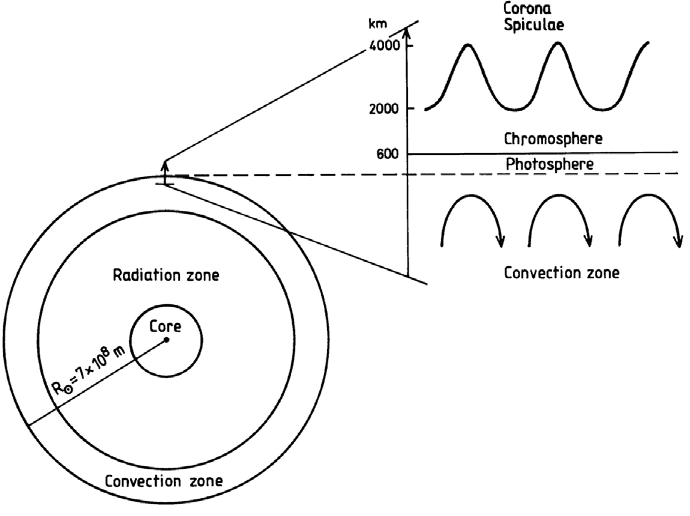
\includegraphics[width=.6\linewidth]{bilder/L9_zones_in_the_sun.png}
    \caption{A schematic diagram showing the different zones of the Sun; the core, the radiation zone and the convection zone.}\label{fig:L9_zones_in_the_sun}
\end{figure}
\begin{figure}[t]
    \centering
    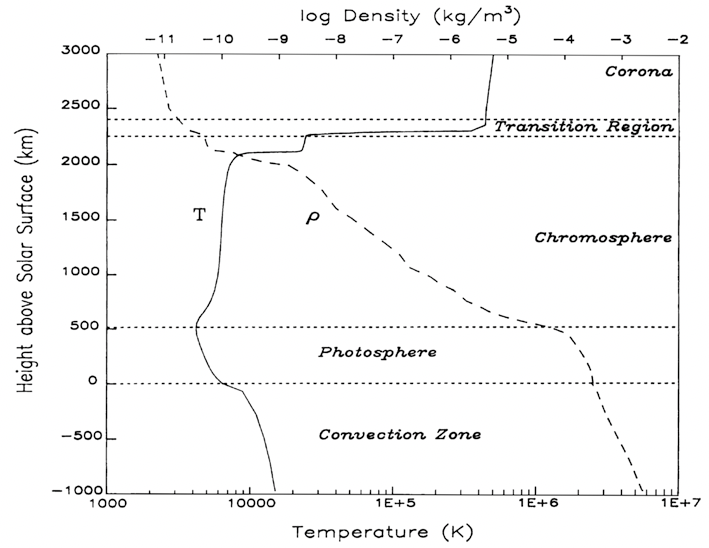
\includegraphics[width=.6\linewidth]{bilder/L9_sun_temperature.png}
    \caption{Temperature and density profiles in the solar atmosphere showing the steep temperature increase in the transition region. The zero level refers to about one solar radius from te center of the solar disk.}\label{fig:L9_sun_temperatures}
\end{figure}

\section{Electromagnetic radiation from the Sun}
The observed radiation spectrum from the Sun as measured from the Earth's surface in the wavelength region \(200\)--\(\SI{3200}{\nano\metre}\) is shown in \cref{fig:L9_sun_spectral_irradiance}. The solar spectrum, as observed outside the Earth's atmosphere, compared to that of a blackbody, give a temperature of \SI{6000}{\kelvin}.

Ultraviolet (UV) and X-ray radiation shorter than 200 nm are strongly absorbed by air. The UV radiation region is usually divided into two parts. (1) the far ultraviolet (FUV) region between 100 and 200 nm coming from the upper photosphere. It is absorbed in the mesosphere/thermosphere. (2) the extreme ultraviolet (EUV) region between 10 and 100 nm coming from the chromosphere. There are some strong emission lines from this, such as the hydrogen Balmer lines at \SI{121.6}{\nano\metre} (\(Ly_\alpha \)), \SI{102.5}{\nano\metre} (\(Ly_\beta \)), etc., the helium line at 58.4 nm and the oxygen line at 130.4 nm.

For spectral irradiance and the variability, we have the largest variabilities for \(\lambda <\SI{300}{\nano\metre}\).
\begin{figure}[t]
    \centering
    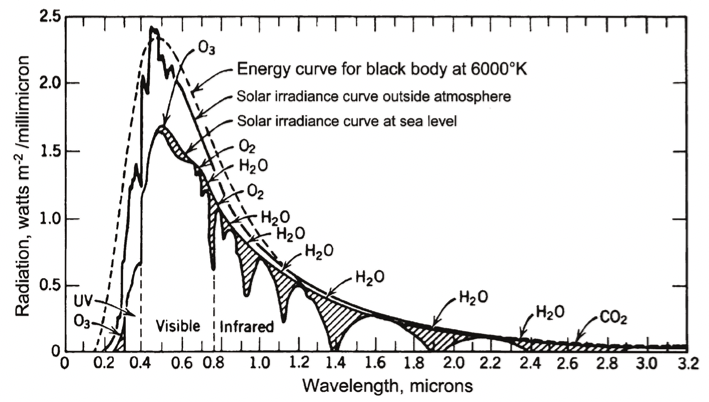
\includegraphics[width=.6\linewidth]{bilder/L9_sun_spectral_irradiance.png}
    \caption{The Sun's spectral irradiance per unit wavelength of solar radiation observed at sea level compared with a blackbody spectrum at \(\num{6000}\) K and the spectrum observed outside the Earth's atmosphere.}\label{fig:L9_sun_spectral_irradiance}
\end{figure}

\section{Planck's radiation law}
Let us assume that the Sun is radiating its energy approximately as a blackbody with temperature \(T\), then the spectral brightness, \(B_\nu \), per frequency band, \(\tn{d}\nu \), according to Planck's radiation law will be
\begin{equation*}
    B_\nu=\frac{2h\nu^3}{c^2}\frac{1}{\exp\left(\frac{h\nu}{kT}\right)-1},\qquad \left[\si{\watt\hertz^{-1}}\tn{sr}^{-1}\si{\metre^{-1}}\right]
\end{equation*}
where \(B_\nu \) is given in the frequency range \(\nu \) to \(\nu+\tn{d}\nu \). We notice that it only depends on the temperature and not the geometry of the body. We can also express the spectral brightness \(B_\lambda \) per unit wavelength band between \(\lambda \) and \(\lambda+\tn{d}\lambda \) in the following manner when noting that \(\tn{d}\nu=-\left(c/\lambda^2\right)\tn{d}\lambda \) and \(B_\nu\tn{d}\nu=B_\lambda\tn{d}\lambda \):
\begin{equation*}
    B_\lambda=\frac{2hc^2}{\lambda^5}\frac{1}{\exp\left(\frac{hc}{k\lambda T}\right)-1}
\end{equation*}
We find that the maximum in \(B_\lambda \) (\(\p{\lambda}{B_\lambda}=0\)) occurs at the wavelength \(\lambda_m\) which satisfies
\begin{equation*}
    5\left(1-e^{-x_m}\right)=x_m
\end{equation*}
where
\begin{equation*}
    x_m=\frac{hc}{k\lambda_m T}
\end{equation*}
The solution can be found numerically to be \(x_m=4.9651\dots \), which then finally gives
\begin{equation*}
    \lambda_{m}T=\num{2.898e-3}\si{\metre\kelvin}
\end{equation*}
which is the \emph{Wien displacement law} expressing that the wavelength at maximum radiation for a blackbody is inversely proportional to the temperature. \Cref{fig:L9_blackbody_radiation} demonstrates the Wien displacement law where \(B_\lambda \) is presented for different temperatures. We had a maximum in the solar spectrum close to \SI{500.0}{\nano\metre} which then gives a temperature of
\begin{equation*}
    T=\SI{5780}{\kelvin}
\end{equation*}

According to the Stefan-Boltzmann law, which is the integrated Planck's equation over all wavelengths and solid angles, we have the total radiated power \(Q\) given by
\begin{equation}\label{eq:L9_stefan_boltzmann}
    Q=qS=\sigma T^4S
\end{equation}
where \(S\) is the surface of the radiating body and \(q\) is the radiated power per unit area. The Stefan-Boltzmann constant \(\sigma \) is given by
\begin{equation*}
    \sigma=\frac{2\pi^5k^4}{15c^2h^3}=\num{5.67e-8}\si{\watt\metre^{-2}\kelvin^{-4}}
\end{equation*}
For the Sun, the radiated power per unit area is
\begin{equation*}
    q_\odot=\sigma T_\odot^4=\num{6.3e7}\si{\watt\metre^{-2}}
\end{equation*}
The total radiated power from the Sun will be
\begin{equation*}
    Q_\odot=4\pi R_\odot^2q_\odot=\num{3.9e26}\si{\watt}
\end{equation*}
The power that is reaching Earth we can find by assuming that the power flux is conserved.
\begin{equation*}
    E_e=q_\odot{\left(\frac{R_\odot}{r}\right)}^2=\SI{1380}{\watt\metre^{-2}}
\end{equation*}
\begin{figure}[t]
    \centering
    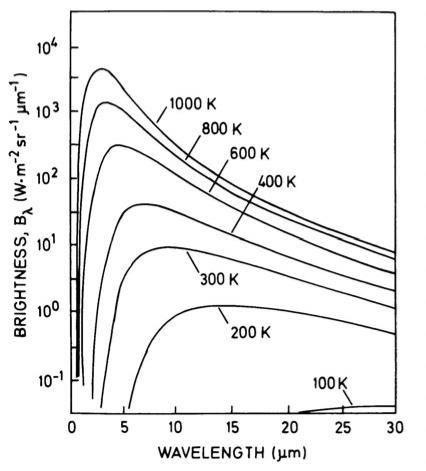
\includegraphics[width=.4\linewidth]{bilder/L9_blackbody_radiation.png}
    \caption{Curves showing blackbody radiation functions for bodies with different temperatures.}\label{fig:L9_blackbody_radiation}
\end{figure}

\section{The greenhouse effect}
The heat radiated from the Sun is the main heat source for the Earth and its atmosphere, but to maintain an equilibrium temperature we need a comparable loss of heat radiation. The blackbody radiation from the Earth is
\begin{equation*}
    Q_e=4\pi R_e^2\sigma T_e^4
\end{equation*}
while the absorption of the radiation from the Sun is
\begin{equation*}
    Q_{se}=\left(1-\alpha\right)E_e\pi R_e^2
\end{equation*}
where \(\alpha \) is the albedo or reflection coefficient (\(\approx 0.3\)). For thermal equilibrium we need \(Q_{se}=Q_e\), but this gives
\begin{equation*}
    T_e={\left(\frac{(1-\alpha)E_e}{4\sigma}\right)}^{1/4}=\SI{255}{\kelvin}
\end{equation*}
I.e.\ we need a green house effect to explain the discrepancy. The average temperature on the surface is \(T_e=288\) K, which according to the Wien displacement law give infrared radiation.

Let us now assume that the atmosphere has a temperature \(T_a\), and that it radiate accordingly. The heat balance we now get is
\begin{equation*}
    \sigma 4\pi R_e^2T_e^4=2\sigma 4\pi R_e^2T_a^4
\end{equation*}
and by solving for \(T_a\) we find
\begin{equation*}
    T_a^4=\frac{1}{2}T_e^4
\end{equation*}

We now include the heat from the sun, and the balance become \(Q_{se}+\frac{1}{2}Q_a=Q_e\), and by insertion we can solve for \(T_e\) and obtain
\begin{equation*}
    T_e={\left[\frac{(1-\alpha)E_e}{2\sigma}\right]}^{1/4}=\SI{304}{\kelvin}
\end{equation*}

\section{Radio wave emissions from the Sun}
For radio frequencies corresponding to the wavelength regime we have \(10^4\)--\(10^2\si{\mega\hertz}\). The energy related to this is typically \(h\nu=\num{6.6e-25}\si{\joule}\). This is much less than the thermal energy for a reasonable solar temperature which corresponds to \(kT_\odot=\num{8.4e-20}\si{\joule}\). Because of this, we can use the Rayleigh-Jeans approximation of Planck's radiation law (\(k\nu\ll kT\))
\begin{equation}\label{eq:L9_rayleigh_jeans}
    B_\nu=\frac{2h\nu^3}{c^2}\frac{1}{1+h\frac{\nu}{kT}+\cdots -1}=\frac{2kT\nu^2}{c^2}
\end{equation}
\Cref{fig:L9_solar_radiowave_radiation_spectrum} show a schematic diagram of the solar radio wave radiation spectrum for a quiet Sun as well as for the slowly varying component (the S-component). (From Tohmatsu, 1990.)

We now look at \cref{fig:L9_sun_earth_geometry}. We notice that the radiation energy emitted from an infinitesimal area \(\tn{d}\sigma \) perpendicular to the Sun-Earth line at a point \(P\) on the Sun and hitting the surface of the Earth is
\begin{equation*}
    \tn{d}I_\nu=B_\nu\tn{d}\sigma\Omega=B_\nu\tn{d}\sigma\frac{S}{r_1^2}
\end{equation*}
where \(S\) is the projection of the surface of the Earth facing the Sun on a plane perpendicular to the line from \(P\) to the Earth's center, \(r_1\) is the distance from \(P\) to the Earth \(r_1\gg R_e\) and \(\Omega=S/r_1^2\) is the solid angle corresponding to the surface \(S\) seen from \(P\). We assume the brightness to be isotropic, and that \(r\gg R_\odot \) so that \(r=r_1\). The total radiation flux per unit area reaching the Earth is then
\begin{equation*}
    \phi_\nu=\frac{I_\nu}{S}=\int_\Sigma B_\nu\frac{\tn{d}\sigma}{r^2}=\pi{\left(\frac{R_\odot}{r}\right)}^2B_\nu
\end{equation*}
where \(\Sigma \) is the Sun's effective area. Substituting in from \cref{eq:L9_rayleigh_jeans} gives
\begin{equation*}
    \phi_\nu=\pi{\left(\frac{R_\odot}{r}\right)}^2\frac{2k}{c^2}\nu^2T=\pi{\left(\frac{R_\odot}{r}\right)}^2\frac{2kT}{\lambda^2}
\end{equation*}
We plug in the proper constants and end up with
\begin{equation}\label{eq:L9_rad_flux}
    \phi_\nu=\num{2.09e-44}\nu^2T\quad \left[\si{\watt\metre^{-2}\hertz^{-1}}\right]
\end{equation}

For the 10.7 cm radio flux we find from \cref{eq:L9_rad_flux} that the radiation flux is given by (\(F_\lambda=\phi_\nu/\nu^2\))
\begin{equation*}
    F_{10.7}=\num{16.4e-26}T
\end{equation*}
and the index is therefore a direct indicator of the effective temperature. The 10.7 is also directly correlated with electron density, hence its importance.

We introduce the electron plasma frequency given by
\begin{equation*}
    f_{pe}=\frac{1}{2\pi}{\left(\frac{n_{e}e^2}{m_{e}\varepsilon_0}\right)}^{1/2}=K\sqrt{n_e}
\end{equation*}
From a given level of the solar atmosphere characterized by a specific electron density of \(n_e\) only radiation with a frequency \(\nu >f_{pe}\) will escape if the influence of the magnetic field is neglected. \Cref{fig:L9_variations_in_electron_density} show that electron density decreases strongly from close to \(10^{15} \si{\metre^{-3}}\) at \(1R_\odot \) to close to \(10^{10} \si{\metre^{-3}}\) at \(10R_\odot \). According to our understanding of the plasma frequency we now realize that by observing radio emissions from the Sun at increasing frequencies (or decreasing wavelengths) we are probing deeper and deeper into the solar atmosphere. It is found that while m-waves are formed far out in the corona, cm-waves are generated deep in the solar atmosphere and mm-waves penetrate almost all the way from the photosphere. 99\% of the energy: \(\lambda=276\)--\(\SI{4960}{\nano\metre}\), 99.9\% of the energy: \(\lambda=217\)--\(\SI{10940}{\nano\metre}\). Only 0.1\% is outside of the visible, IR and UV\@.
\begin{figure}[t]
    \centering
    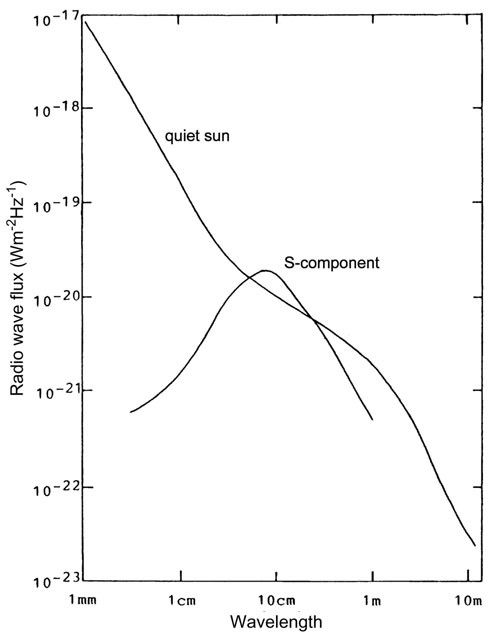
\includegraphics[width=.4\linewidth]{bilder/L9_solar_radiowave_radiation_spectrum.jpg}
    \caption{Schematic diagram of the solar radiowave radiation spectrum for a quiet Sun as well as for the slowly varying component (the \(S\)-component).}\label{fig:L9_solar_radiowave_radiation_spectrum}
\end{figure}
\begin{figure}[t]
    \centering
    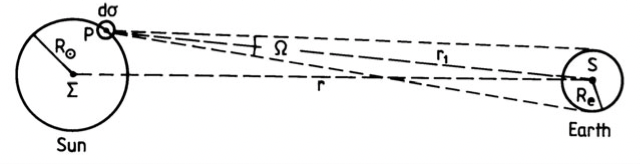
\includegraphics[width=.9\linewidth]{bilder/L9_sun_earth_geometry.png}
    \caption{The Sun–Earth geometry where \(S\) is the projection of the Earth's surface to a plane perpendicular to the Sun-Earth line, \(r\) is equal to 1 AU, and \(\tn{d}\sigma \) is the projection of an infinitesimal area on to a plane perpendicular to the line from a point \(P\) on the Sun to the Earth's center. Since \(r\gg R_\odot \), where \(R_\odot \) is the solar radius, \(r_1\) can be considered equal to \(r\).}\label{fig:L9_sun_earth_geometry}
\end{figure}
\begin{figure}[t]
    \centering
    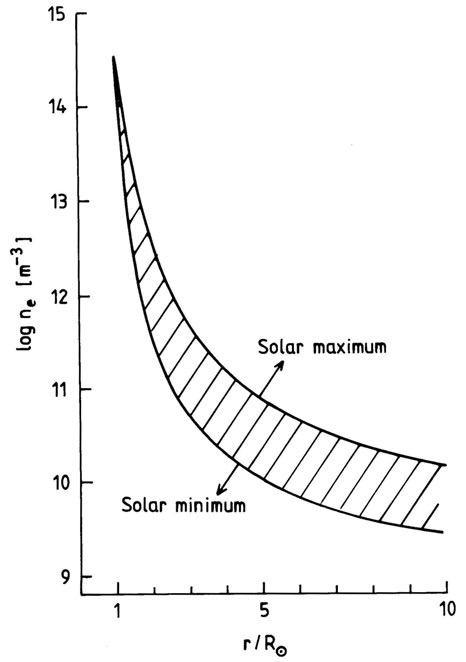
\includegraphics[width=.4\linewidth]{bilder/L9_variations_in_electron_density.jpg}
    \caption{Variations in electron density in the solar atmosphere from the base of the photosphere to a distance of 10 \(R_\odot \) from the center of the solar disk under different solar activity conditions.}\label{fig:L9_variations_in_electron_density}
\end{figure}

\section{Sunspots \& the solar cycle}
A sunspot was first observed by Galileo. The solar cycles have a period of on average eleven years.

The fact that sunspots come and go in cycles was not appreciated until 1843. After some time, Wolf devised a quantitative definition for a sunspot number and studied sunspot data for the years 1700 to 1848. In its present form the Wolf sunspot number \(R_z\) is defined as
\begin{equation}\label{eq:L9_wolf_sunspot_number}
    R_z=k\left(10g+f\right)
\end{equation}
where \(f\) is the total number of sunspots regardless of size, \(g\) is the number of sunspot groups and \(k\) is a normalization constant accounting for the different observatories.

\section{Electromagnetic radiation from a disturbed Sun}
The most short-lived phenomenon observed from Earth on the solar surface is the flare event which usually occurs within a region encompassed by a large magnetically complex bipolar sunspot group.

Let us assume by inspecting \cref{fig:L9_variations_in_electron_density} that the electron density at a distance \(z\) from the solar surface is
\begin{equation*}
    n_e(z)=n_{e0}\exp\left(-\frac{z-z_0}{H}\right)
\end{equation*}
where \(n_{e0}\) is the electron density at a reference height \(z_0\) and \(H\) is the \(e\)-folding scale height. From the expression of plasma frequency we find
\begin{equation*}
    \fracd{f_{pe}}=K\frac{1}{2}n_e{(z)}^{-1/2}\fracd[z]{n_e(z)}\fracd{z}=-\frac{f_{pe}}{2H}\fracd{z}
\end{equation*}
and the propagation velocity \(v_{RS}\) of the radio source emitting a radio frequency \(f\) equal to the instantaneous plasma frequency \(f_{pe}\) is given by
\begin{equation*}
    v_{RS}=\fracd{z}=-2H\fracd{}\ln f
\end{equation*}
During the first minutes of development after the flare flash has occurred, groups of very narrow bursts appear that show a fast drift from high to low frequency.
\begin{enumerate}
    \item [\emph{Type III}] Right after the flare, narrow, fast relativistic electrons in the corona, \(v=0.2\)--\(0.9c\). Originate at \(50\)--\(100 R_\odot \)
    \item [\emph{Type V}] 1--3 min after Type III
    \item [\emph{Type II}] Slower, last 5--10 min, appears 5 min after Type III, \(v=500\)--\(1500\si{\kilo\metre/\second}\), EM shock waves
    \item [\emph{Type IV}] A broad continuum, 10 min to hours. Trapped relativistic particles
    \item [\emph{Type I}] Hours to days. Not related to flares. Might be caused by large sunspots
\end{enumerate}

\section{Particle emissions from the Sun}
A quiet Sun radiates not only electromagnetic waves, but also particles. A solar wind is always blowing. This wind is not a steady wind, but rather gusty as it varies quite strongly in velocity as well as density at a distance from the Sun corresponding to the Earth’s orbit.

Under quiet conditions the wind has a medium velocity of \SI{400}{\kilo\metre/\second} but can, however, vary between 200 and \SI{700}{\kilo\metre/\second} (takes 1--5 days to the Earth). The density is often between \(10^6\) and \(\num{2e7}\si{\metre^{-3}}\). The average energy of the protons is of the order of 1 keV while the electrons have energies of the order of 1 eV. The average particle flux from the Sun can be estimated to be
\begin{equation*}
    \phi=nv\approx\num{2e12}\si{\metre^{-2}\second^{-1}}
\end{equation*}
Total average particle loss per unit time form the Sun is therefore
\begin{equation*}
    \p{t}{N}=4\pi R_\odot^2\phi\approx\num{1.23e31}\si{\second^{-1}}
\end{equation*}
By neglecting the mass of the electrons in the solar wind, this particle loss per unit time corresponds to a mass loss per unit time given by
\begin{equation*}
    \p{t}{m}=\p{t}{N}m_p=\num{2.21e5}\si{\kilo\gram/\second}
\end{equation*}
which is a loss much smaller than what we have from radiation (\(\num{4.3e9}\si{\kilo\gram/\second}\)). The proton temperature in the solar wind is \(10^4\)--\(\num{2e5}\si{\kelvin}\) while the electron temperature is a factor of 3--4 larger. The magnetic field strength varies between 1 and \SI{15}{\nano\tesla}, where on average we have \(T_{||}\approx 2T_\perp \).

Of the characteristic parameters we have given for the solar wind so far, we notice that the speed of sound of the solar wind gas is approximately
\begin{equation*}
    C_s=\sqrt{\frac{\gamma kT_\odot}{m_p}}=\num{1.17e4}\si{\metre/\second}
\end{equation*}
where \(\gamma=5/3\) is the adiabatic constant and \(T_\odot=10^4\) K. Since the solar wind is on average 30 times higher, the solar wind is supersonic. The place where the solar wind turns subsonic due to pressure forces from the interstellar medium is called the heliopause.

\section{Fluid flow in a nozzle}
Let an incompressible gas with density \(\rho \) stream through a tube with a varying cross-section \(A\). Since mass flux through any cross-section of the tube must be constant, we have
\begin{equation*}
    \phi_m=A\rho v=\tn{const}
\end{equation*}

The pressure gradient will be balanced by the inertia force when no other forces are acting in the equation of motion. Considering only one dimension along \(r\) we have
\begin{equation*}
    \fracd{p}=-\rho\fracd{v}=-\rho\fracd[r]{v}v
\end{equation*}
Using \(\tn{d}p=-\rho v\tn{d}v\), we can plug this into our expression. Thus
\begin{align}
    \frac{\tn{d}p}{\rho}=\fracd[\rho]{p}\frac{\tn{d}\rho}{\rho}=-v\tn{d}v\notag \\
    \Rightarrow \frac{\tn{d}\rho}{\rho}=-v\tn{d}v{\left(\fracd[\rho]{p}\right)}^{-1}\label{eq:L9_change_in_rho}
\end{align}
For adiabatic processes we have \(p\rho^{-\gamma}=\tn{const}\), so we get
\begin{equation}\label{eq:L9_sound_speed_relation}
    \rho^{-\gamma}\tn{d}p-\gamma p\rho^{-\gamma-1}\tn{d}\rho=0\Rightarrow\fracd[\rho]{p}=\gamma\frac{p}{\rho}=C_s^2
\end{equation}
where \(C_s\) is the sound speed, and we can plug this into \cref{eq:L9_change_in_rho}. Conservation of mass flux means \(\tn{d}\phi_m=0\), i.e.
\begin{align*}
    \frac{\tn{d}\phi_m}{\phi_m}=\frac{\tn{d}A}{A}+\frac{\tn{d}\rho}{\rho}+\frac{\tn{d}v}{v}=0\\
    \frac{\tn{d}A}{A}-\frac{v}{C_s^2}\tn{d}v+\frac{\tn{d}v}{v}=0\\
    \frac{\tn{d}A}{A}=\left(\frac{v^2}{C_s^2}-1\right)\frac{\tn{d}v}{v}
\end{align*}
If \(v\) is supersonic from the start, then \(v\) has to decrease as long as \(A\) decreases, and \(v\) will become subsonic. If, on the other hand, \(v\) is subsonic at the start it can only increase and become supersonic if \(v=c_s\) when \(\tn{d}A=0\) and the cross-section increases again. This is illustrated in \cref{fig:L9_mass_flow_through_nozzle}. If, however, the gas is streaming so slowly that it does not reach the speed of sound at the narrowest part of the tube, the speed of the gas will then continue to decrease as it passes through the throttle.
\begin{figure}[t]
    \centering
    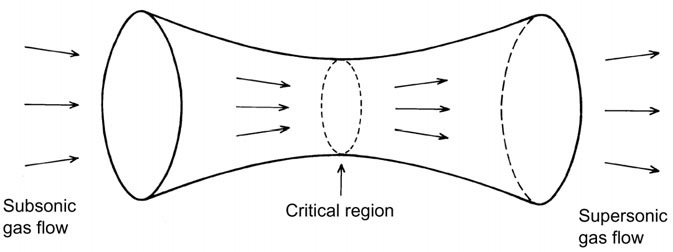
\includegraphics[width=.8\linewidth]{bilder/L9_mass_flow_through_nozzle.jpg}
    \caption{Mass flow through a nozzle with a minimum cross-section to explain the presence of a critical region in the mass flow in order for the flow speed to become supersonic.}\label{fig:L9_mass_flow_through_nozzle}
\end{figure}

\section{The solar wind equation}
We will now assume that the coronal gas is an ideal and incompressible gas and that we can treat it as a hydrodynamic fluid. This means that the collisions are frequent enough that local thermodynamic equilibrium is maintained. We will in the following treatment neglect viscosity and magnetism and limit ourself only to pressure, internal forces, and gravity. Then \cref{eq:L9_change_in_rho} can be written
\begin{equation*}
    \frac{\tn{d}p}{\rho}=\fracd[\rho]{p}\frac{\tn{d}\rho}{\rho}=-v\tn{d}v-\frac{GM_\odot}{r^2}\tn{d}r
\end{equation*}
where \(r\) is the radial distance from the Sun. We plug in in \cref{eq:L9_sound_speed_relation} and divide by \(C_s^2\) to obtain
\begin{equation*}
    \frac{\tn{d}\rho}{\rho}=-\frac{v}{C_s^2}\tn{d}v-\frac{GM_\odot}{C_s^2}\frac{\tn{d}r}{r^2}
\end{equation*}
Using again conservation of flux we have
\begin{equation*}
    \frac{\tn{d}\rho}{\rho}=-\left(\frac{\tn{d}A}{A}+\frac{\tn{d}v}{v}\right)
\end{equation*}
Inserting for \(\tn{d}\rho/\rho \) and solving for \(\tn{d}A/A\) we get
\begin{equation*}
    \frac{\tn{d}A}{A}=\left(\frac{v^2}{C_s^2}-1\right)\frac{\tn{d}v}{v}+\frac{GM_\odot}{C_s^2}\frac{\tn{d}r}{r^2}
\end{equation*}
The solar wind is expanding spherically and symmetrically so that
\begin{equation*}
    \frac{\tn{d}A}{A}=\frac{2}{r}\tn{d}r
\end{equation*}
which leads us to the relationship
\begin{equation*}
    \left(2-\frac{GM_\odot}{C_s^2}\frac{1}{r}\right)\frac{\tn{d}r}{r}=\left(\frac{v^2}{C_s^2}-1\right)\frac{\tn{d}v}{v}
\end{equation*}
and finally
\coloredeq{eq:L9_critical_distance}{2\left(1-\frac{r_c}{r}\right)\frac{\tn{d}r}{r}=\left(\frac{v^2}{C_s^2}-1\right)\frac{\tn{d}v}{v}}
where \(r_c=GM_\odot/2C_s^2\) is the so-called critical distance. There are several solutions to \cref{eq:L9_critical_distance}, with a geometrical view of it in \cref{fig:L9_solution_solar_wind_equation}. The important solution for us is; if the wind starts out from the Sun with an increasing velocity which initially is smaller than \(C_s\), then both sides in \cref{eq:L9_critical_distance} are negative. When \(r\) equals the critical distance \(r_c\), the left-hand side is zero and therefore the right-hand side has to be zero also (i.e., \(v=C_s\)). If \(v=C_s\) at the critical distance, then \(v\) can continue to accelerate to a supersonic speed.
\begin{figure}[t]
    \centering
    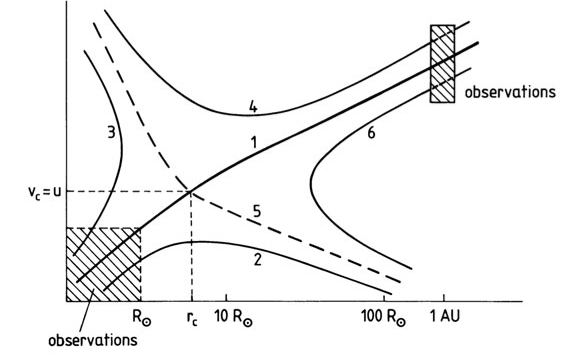
\includegraphics[width=.6\linewidth]{bilder/L9_solution_solar_wind_equation.png}
    \caption{Alternative solutions of the solar wind equation explained in the text.}
    \label{fig:L9_solution_solar_wind_equation}
\end{figure}

\section{The frozen-in field concept}
Observed features that support the existence of solar magnetic field are the loop prominences observed in the \(H_\alpha \) line. Tentative measurements give magnetic fields of the order of \(\num{5e-3}\si{\tesla}\). The loops typically lasts for about 20 minutes.

The current density for a true conducting fluid is given by \(\gf{j}'=\sigma\gf{E}'\) in a frame moving with the plasma. Due to the high conductivity, we need not express it as a tensor but merely as a scalar. From Ohm's law we have \(\gf{j}=\sigma\gf{E}'=\sigma\left(\gf{E}+\gf{v}\times\gf{B}\right)\). When \(\sigma\rightarrow\infty \) we get \(\gf{E}=-\gf{v}\times\gf{B}\). Faraday's law tells us that
\begin{equation*}
    \p{t}{\gf{B}}=-\nabla\times\gf{E}=\nabla\times\left(\gf{v}\times\gf{B}\right)
\end{equation*}
If we now consider the time the variation of the magnetic flux through a surface moving with velocity \(v\)
\begin{equation*}
    \fracd{\phi}=\iint_S\p{t}{\gf{B}}\cdot\tn{d}\gf{s}+\oint_L\gf{B}\cdot\left(\gf{v}\times\tn{d}\gf{\ell}\right)
\end{equation*}
where \(S\) is the surface and \(L\) is a closed loop encircling this surface. The second term can be rewritten using Gauss' law, hence
\begin{eqnarray}
    \fracd{\phi}=\iint_S\left[\p{t}{\gf{B}}-\nabla\times\left(\gf{v}\times\gf{B}\right)\right]\tn{d}\gf{s}
\end{eqnarray}
We know from before that \(\tn{d}\phi/\tn{d}t=0\) so that \(\phi \) is a constant. The flux through the surface is kept, and the magnetic field is therefore frozen-in. Remember, however, that strictly speaking this is correct only when \(v\ll c\).

\section[The garden hose effect]{The garden hose effect (AB 1.13)}
Let us assume that the plasma leaves the solar surface in the equatorial plane at a distance \(r_0\) from the solar center. Then, after a time, \(t\), the position of the plasma in the same plane can be described as
\begin{align*}
    r&=vt+r_0\\
    \phi&=\Omega t+\phi_0
\end{align*}
where \(\phi_0\) is the longitude on the Sun from which the plasma emerges, \(\Omega \) is the angular velocity of the Sun, and \(v\) is the solar wind velocity. Eliminating \(t\) gives
\begin{equation*}
    r=v\frac{\phi-\phi_0}{\Omega}+r_0
\end{equation*}
which is the equation for an Archimedean spiral as can be seen in \cref{fig:L9_garden_hose}.
\begin{figure}[t]
    \centering
    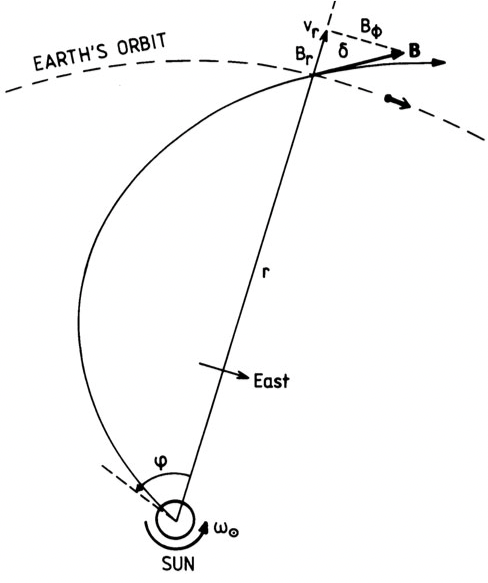
\includegraphics[width=.4\linewidth]{bilder/L9_garden_hose.png}
    \caption{Solar wind plasma streams radially out from a rotating Sun, and its motion can be described as an Archimedean spiral (garden hose). At the position of the Earth the angle (\(\delta \)) between the plasma velocity and the Sun–Earth line is close to \SI{45}{\degree}. The Earth’s orbit is indicated.}\label{fig:L9_garden_hose}
\end{figure}

As the plasma will now drag the magnetic field along, it will follow the same trajectory and form similar spirals. Introducing polar coordinates and still confining ourself to the equatorial plane, we have
\begin{align*}
    \gf{v}&=\left(v_r,v_\phi\right)\rightarrow v(r)\\
    \gf{B}&=\left(B_r,B_\phi\right)\rightarrow B(r)
\end{align*}
I.e.\ we say that the magnitude of the solar wind velocity and the magnetic field depend only of the radial distance from the Sun. In spherical coordinates we then have
\begin{equation*}
    \nabla\cdot\gf{B}=\frac{1}{r^2}\p{r}{\left(r^2B_r\right)}=0
\end{equation*}
or \begin{equation*}
    r^2B_r=r_0^2B_0=\tn{const} \Leftrightarrow B_r=B_0{\left(\frac{r_0}{r}\right)}^2
\end{equation*}
where \(B_0\) is the magnetic field at a reference point at the solar surface.

Since \(\p{t}{B}=0\) and the frozen-in concept apply we have
\begin{eqnarray}
    \nabla\times\left(\gf{v}\times\gf{B}\right)=0
\end{eqnarray}
which in spherical coordinates reads
\begin{equation*}
    \frac{1}{r}\p{r}{\left[r\left(v_\phi B_r-v_{r}B_\phi\right)\right]}=0
\end{equation*}
\begin{equation*}
    \Rightarrow r\left(v_\phi B_r-v_{r}B_\phi\right)=\tn{const}
\end{equation*}
If we assume that \(\gf{B}\) is radial at the reference point
\begin{equation}\label{eq:L9_radial_B_sun}
    r_0v_{\phi_0}B_0=rv_\phi B_r-rv_{r}B_\phi
\end{equation}
Since the gas is rotating with the rotation speed of the Sun, we find at the surface of the Sun
\begin{equation*}
    v_{\phi_0}=r_0\Omega
\end{equation*}
We insert this into \cref{eq:L9_radial_B_sun} which yields
\begin{equation*}
    r_0^2\Omega B_0=rv_\phi B_r-rv_{r}B_\phi
\end{equation*}
Solving for \(B_\phi \) give
\begin{equation*}
    B_\phi=\frac{v_\phi-r\Omega}{v_r}B_r
\end{equation*}
For very large distances \(r\Omega > v_\phi \) then
\begin{equation*}
    B_\phi=-\frac{r\Omega}{v_r}B_r=-\frac{r_0^2\Omega}{rv_r}B_0
\end{equation*}
The azimuthal component therefore decreases with distance from the Sun as \(1/r\) (more slowly than the radial component).

The angle the magnetic field will form with the radius vector to the Sun is
given by (\cref{fig:L9_garden_hose})
\begin{equation*}
    \tan\delta=\left|\frac{B_\phi}{B_r}\right|=\frac{r\Omega}{v}
\end{equation*}
for large distances. Plugging in some numbers (\(r=\)1 AU, \(\Omega=2\pi/T\), \(T=24.7\) days, \(v=\SI{400}{\kilo\metre/\second}\)) gives \(\tan\delta\approx 1\Rightarrow \delta\approx\SI{45}{\degree}\). So the ``garden hose'' angle is approximately \SI{45}{\degree}
\begin{figure}[t]
    \centering
    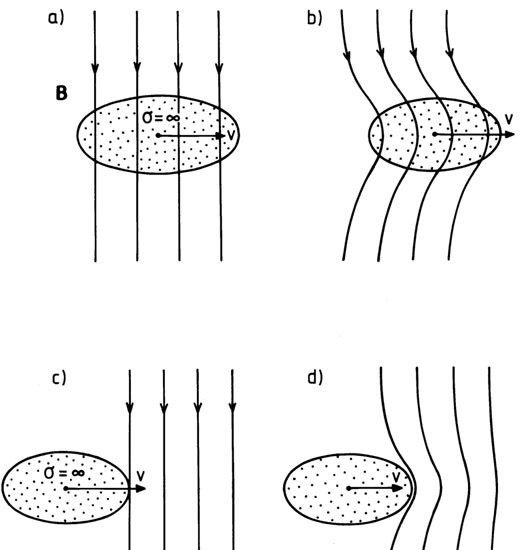
\includegraphics[width=.4\linewidth]{bilder/L9_froze_in.jpg}
    \caption{An illustration of the frozen-in field concept. (a) A magnetic field \(\gf{B}\) is assumed to be penetrating a region of highly conducting plasma. (b) When the plasma starts to move, the magnetic field lines will be frozen-in and follow the motion of the plasma. (c) A highly conducting plasma is approaching an area of the magnetic field. (d) Due to the high conductivity the field cannot penetrate the plasma and is pushed ahead of the plasma blob.}\label{fig:L9_frozen_in}
\end{figure}

\section{Coronal mass ejections (CME)}
This is massive bursts of solar wind and magnetic fields that is released into space. They come from active regions on the Sun’s surface (groupings of sunspots), and at solar max there are \(\sim 3\) per day and at solar min \(\sim 0.2\) per day.